To generate all execution graphs that correspond to the given CGraph, we build one universal directed acyclic graph that includes all equivalent execution graphs and then extract them.

We represent graph as adjacency list, implemented as a map:

\begin{lstlisting}[language=Haskell]
data Node =
    Source NodeName
  | Op1 NodeName NodeId
  | Op2 NodeName NodeId NodeId

newtype Graph = Graph (Map NodeId Node)
\end{lstlisting}

% We represent the graph as an adjacency list of nodes. Each node includes 

We build a universal graph iteratively.
In the first step, we add all environment sources to the universal graph and the sources list.
In the next one, we consider all available sources and operations, and if some sources satisfy input contracts of some operation, we add this operation to the universal graph with unique id and to the sources list.
The number of steps should be one more than the number of operations to ensure that the universal graph includes all graphs that correspond to the CGraph because, in this case, the longest possible path in the graph includes all available operations.

To extract all graphs corresponding to the CGraph, firstly for each operation of semantics we find corresponding ids in the universal graph.
Then we calculate a cartesian product of all this id sets.
Each element of the cartesian product includes ids that correspond to all of the semantics operations.
For each such element, we extract an execution graph from the universal graph, which leafs have elements' ids.
Finally, we filter graphs that do not have duplicated nodes.
These extracted graphs form a set of all equivalent graphs for the given task.

On the Figure~\ref{fig:gen} we show a generation example for the graph shown on the Figure~\ref{fig:example}.
Purple nodes correspond to the fraud metric semantics node, orange~--- to the participants semantics node.
Nodes with red frames represent an extracted graph.

\begin{figure}
    \flushright
    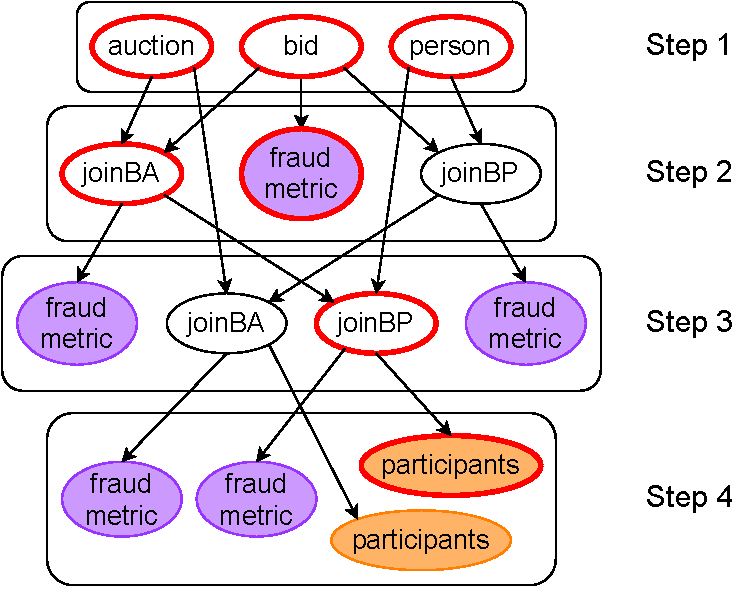
\includegraphics[width=0.4\textwidth]{images/generation}
    \caption{Generation example of the running example graph.}
    \label{fig:gen}
\end{figure}

We use some tricks to make graphs generation faster.
Firstly, we keep a set of its predecessor operations for each source to filter the following operations (each execution graph cannot have node copies).
Secondly, we keep a set of the generated nodes to avoid adding the same nodes with different ids later.

% \begin{lstlisting}[language=Haskell]
% extract :: Graph -> Set NodeId -> Graph
% findIds :: Graph -> NodeName -> [NodeId]
% cartesianProduct :: [[a]] -> [[a]]

% semanticNids 
%   :: Graph -> Semantics -> [Set NodeId]
% semanticNids g = 
%     map Set.fromList . cartesianProduct 
%   . map (findIds g) . Set.toList

% genGraphs :: ( InCont s i, OutCont s o
%              , OutCont1 s o1, OutCont2 s o2) 
%           => CGraph i o o1 o2 -> [Graph]
% genGraphs (e, semantics) = 
%   let bigGraph = ... in
%   let graphs = 
%           map (bigGraph `extract`) 
%         $ semanticNids bigGraph semantics in
%   filter Graph.noSameNodes graphs
% \end{lstlisting}
